\documentclass{beamer}
\usepackage[utf8]{inputenc}

\usetheme{Madrid}
\usecolortheme{default}
\usepackage{amsmath,amssymb,amsfonts,amsthm}
\usepackage{txfonts}
\usepackage{tkz-euclide}
\usepackage{listings}
\usepackage{adjustbox}
\usepackage{array}
\usepackage{tabularx}
\usepackage{gvv}
\usepackage{lmodern}
\usepackage{circuitikz}
\usepackage{tikz}
\usepackage{graphicx}

\setbeamertemplate{page number in head/foot}[totalframenumber]

\usepackage{tcolorbox}
\tcbuselibrary{minted,breakable,xparse,skins}



\definecolor{bg}{gray}{0.95}
\DeclareTCBListing{mintedbox}{O{}m!O{}}{%
  breakable=true,
  listing engine=minted,
  listing only,
  minted language=#2,
  minted style=default,
  minted options={%
    linenos,
    gobble=0,
    breaklines=true,
    breakafter=,,
    fontsize=\small,
    numbersep=8pt,
    #1},
  boxsep=0pt,
  left skip=0pt,
  right skip=0pt,
  left=25pt,
  right=0pt,
  top=3pt,
  bottom=3pt,
  arc=5pt,
  leftrule=0pt,
  rightrule=0pt,
  bottomrule=2pt,
  toprule=2pt,
  colback=bg,
  colframe=orange!70,
  enhanced,
  overlay={%
    \begin{tcbclipinterior}
    \fill[orange!20!white] (frame.south west) rectangle ([xshift=20pt]frame.north west);
    \end{tcbclipinterior}},
  #3,
}
\lstset{
    language=C,
    basicstyle=\ttfamily\small,
    keywordstyle=\color{blue},
    stringstyle=\color{orange},
    commentstyle=\color{green!60!black},
    numbers=left,
    numberstyle=\tiny\color{gray},
    breaklines=true,
    showstringspaces=false,
}
%------------------------------------------------------------

\title
{2.9.19}
\date{August 31,2025}
\author 
{AI25BTECH11003 - Bhavesh Gaikwad}



\begin{document}


\frame{\titlepage}
\begin{frame}{Question}
 Let $\overrightarrow{a}$,
$\overrightarrow{b}$, and $\overrightarrow{c}$ be three vectors such that $|\overrightarrow{a}|$ = 1, $|\overrightarrow{b}|$ = 2, and $|\overrightarrow{c}|$ = 3. If the
projection of $\overrightarrow{b}$ along $\overrightarrow{a}$ is equal to the projection of $\overrightarrow{c}$ along $\overrightarrow{a}$, and $\overrightarrow{b}$ and $\overrightarrow{c}$ are perpendicular to each other, then find $|3\overrightarrow{a} - 2\overrightarrow{b} + 2\overrightarrow{c}|$.
\end{frame}


\begin{frame}[fragile]
    \frametitle{Theoretical Solution}
Given: 
\begin{equation}
\norm{\vec{a}} = 1, \, \norm{\vec{b}} = 2, \, \norm{\vec{c}} = 3\\
\end{equation}

\begin{equation}
\text{The projection of} \, \vec{b} \, \text{along} \, \vec{a} = \vec{b}^T\dfrac{\vec{a}}{\norm{\vec{a}}^2}\vec{a}    
\end{equation}

\begin{equation}
\text{The projection of} \, \vec{c} \, \text{along} \, \vec{a} = \vec{c}^T\dfrac{\vec{a}}{\norm{\vec{a}}^2}\vec{a}    
\end{equation}


\begin{equation}
\vec{b}^T\dfrac{\vec{a}}{\norm{\vec{a}}}\vec{a} = \vec{c}^T\dfrac{\vec{a}}{\norm{\vec{a}}}\vec{a}\\
\end{equation}

\begin{equation}
\text{Since, } \norm{\vec{a}} = 1
\Rightarrow \quad
\therefore \, \, \vec{b}^T\vec{a} = \vec{c}^T\vec{a}
\end{equation}

Since $\vec{b}$ and $\vec{c}$ are perpendicular: 
\begin{equation}
\vec{b}^T\vec{c} = 0\\
\end{equation}

\end{frame}

\begin{frame}[fragile]
    \frametitle{Theoretical Solution}
\begin{equation}
\text{Let} \, \,\vec{v} = 3\vec{a} - 2\vec{b} + 2\vec{c}
\end{equation}


\begin{equation}
\norm{\vec{v}}^2 = (3\vec{a} - 2\vec{b} + 2\vec{c})^T(3\vec{a} - 2\vec{b} + 2\vec{c})
\end{equation}

\begin{equation}
\norm{\vec{v}}^2 = 9(\vec{a}^T\vec{a}) -6(\vec{a}^T\vec{b}) +6(\vec{a}^T\vec{c}) - 6(\vec{b}^T\vec{a}) + 4(\vec{b}^T\vec{b}) -4(\vec{b}^T\vec{c})+ 6(\vec{c}^T\vec{a}) - 4(\vec{c}^T\vec{b}) + 4(\vec{c}^T\vec{c})\\
\end{equation}


\begin{equation}
    \text{Since} \,  \vec{a}^T\vec{b} = \vec{b}^T\vec{a} \, \text{\&}
\, \vec{a}^T\vec{c} = \vec{c}^T\vec{a}
\end{equation}


\begin{equation}
\norm{\vec{v}}^2 = 9(\vec{a}^T\vec{a}) + 4(\vec{b}^T\vec{b}) + 4(\vec{c}^T\vec{c}) - 12(\vec{a}^T\vec{b}) + 12(\vec{a}^T\vec{c}) - 8(\vec{b}^T\vec{c})
\end{equation}\\
\end{frame}

\begin{frame}[fragile]
\frametitle{Theoretical  Solution}
From Equation 1 \& 6,
\begin{equation}
\vec{a}^T\vec{a} = \norm{\vec{a}}^2 = 1, \,\,
\vec{b}^T\vec{b} = \norm{\vec{b}}^2 = 4, \,\,
\vec{c}^T\vec{c} = \norm{\vec{c}}^2 = 9, \,\,
\vec{b}^T\vec{c} = 0
\end{equation}


\begin{equation}
\norm{\vec{v}}^2 = 9 + 16 + 36
\end{equation}


\begin{align}
    \centering
    \norm{\vec{v}}^2 = 61 
    \quad \Rightarrow \quad
    \norm{\vec{v}} = \sqrt{61}
\end{align}

\begin{align}
\centering
\boxed{\norm{3\vec{a} - 2\vec{b} + 2\vec{c}} = \sqrt{61}}
\end{align}
\end{frame}

\begin{frame}[fragile]
    \frametitle{Python + C Code}
    \begin{lstlisting}
#include <stdio.h>
#include <stdlib.h>
#include <math.h>
#include "libs/geofun.h"
#include "libs/matfun.h"

// Function to save vectors to file
void saveVectorsToFile(double **a, double **b, double **c, double **result, const char *filename) {
    FILE *fp = fopen(filename, "w");
    if (fp == NULL) {
        printf("Error opening file!\n");
        return;
    }
    \end{lstlisting}
\end{frame}


\begin{frame}[fragile]
    \frametitle{Python + C Code}
    \begin{lstlisting}   
    fprintf(fp, "# Vector data for the problem\n");
    fprintf(fp, "# Format: vector_name x y z\n");
    fprintf(fp, "a %.6f %.6f %.6f\n", a[0][0], a[1][0], a[2][0]);
    fprintf(fp, "b %.6f %.6f %.6f\n", b[0][0], b[1][0], b[2][0]);
    fprintf(fp, "c %.6f %.6f %.6f\n", c[0][0], c[1][0], c[2][0]);
    fprintf(fp, "result %.6f %.6f %.6f\n", result[0][0], result[1][0], result[2][0]);
    fprintf(fp, "# Magnitude of result vector: %.6f\n", Matnorm(result, 3));
    
    fclose(fp);
}

// Function to compute 3a - 2b + 2c
double **computeResult(double **a, double **b, double **c) {
    double **scaled_a = Matscale(a, 3, 1, 3.0);
    double **scaled_b = Matscale(b, 3, 1, -2.0);
    double **scaled_c = Matscale(c, 3, 1, 2.0);
    \end{lstlisting}
\end{frame}


\begin{frame}[fragile]
    \frametitle{Python + C Code}
    \begin{lstlisting}
       double **temp = Matadd(scaled_a, scaled_b, 3, 1);
    double **result = Matadd(temp, scaled_c, 3, 1);
    
    freeMat(scaled_a, 3);
    freeMat(scaled_b, 3);
    freeMat(scaled_c, 3);
    freeMat(temp, 3);
    
    return result;
}

// Function exported for Python to use
double compute_vector_magnitude(double *a, double *b, double *c) {
    // Create matrix representations
    double **vec_a = createMat(3, 1);
    double **vec_b = createMat(3, 1);
    double **vec_c = createMat(3, 1);
    \end{lstlisting}
\end{frame}



\begin{frame}[fragile]
    \frametitle{Python + C Code}
    \begin{lstlisting}
       
    for (int i = 0; i < 3; i++) {
        vec_a[i][0] = a[i];
        vec_b[i][0] = b[i];
        vec_c[i][0] = c[i];
    }
    
    double **result = computeResult(vec_a, vec_b, vec_c);
    double magnitude = Matnorm(result, 3);
    
    freeMat(vec_a, 3);
    freeMat(vec_b, 3);
    freeMat(vec_c, 3);
    freeMat(result, 3);
    
    return magnitude;
}
\end{lstlisting}
\end{frame}

\begin{frame}[fragile]
    \frametitle{Python + C Code}
    \begin{lstlisting}
int main() {
    printf("Solving: Find |3a - 2b + 2c| where |a|=1, |b|=2, |c|=3\n");
    printf("Conditions: proj_a(b) = proj_a(c) and b L c\n\n");
    
    // Create specific vectors that satisfy the given conditions
    // Let a = (1, 0, 0) - unit vector along x-axis
    double **a = createMat(3, 1);
    a[0][0] = 1.0; a[1][0] = 0.0; a[2][0] = 0.0;
    
    // For b and c to have equal projections along a and be perpendicular:
    // b*a = c*a and b*c = 0
    // Choose vectors that satisfy these conditions properly:
    
    double k = 0.5; // projection value
    \end{lstlisting}
\end{frame}

\begin{frame}[fragile]
    \frametitle{Python + C Code}
    \begin{lstlisting}
     // b = (k, sqrt(4-k^2), 0)
    double **b = createMat(3, 1);
    b[0][0] = k;
    b[1][0] = sqrt(4 - k*k);
    b[2][0] = 0.0;
    
    // c = (k, m, n) where b*c = 0 and |c| = 3
    // From b*c = 0: k*k + m*sqrt(4-k^2) = 0
    // So m = -k*k/sqrt(4-k^2)
    double **c = createMat(3, 1);
    c[0][0] = k;
    c[1][0] = -k*k / sqrt(4 - k*k);
    
    // n^2 = 9 - k^2 - m^2
    double m = c[1][0];
    double n_squared = 9 - k*k - m*m;
    c[2][0] = sqrt(n_squared);
    \end{lstlisting}
\end{frame}

\begin{frame}[fragile]
    \frametitle{Python + C Code}
    \begin{lstlisting}
         printf("Vector a: ");
    printMat(a, 3, 1);
    printf("Magnitude of a: %.6f\n\n", Matnorm(a, 3));
    
    printf("Vector b: ");
    printMat(b, 3, 1);
    printf("Magnitude of b: %.6f\n\n", Matnorm(b, 3));
    
    printf("Vector c: ");
    printMat(c, 3, 1);
    printf("Magnitude of c: %.6f\n\n", Matnorm(c, 3));
    
    // Verify conditions
    printf("Verification of conditions:\n");
    printf("b*a = %.6f\n", Matdot(b, a, 3));
    printf("c*a = %.6f\n", Matdot(c, a, 3));
    printf("b*c = %.6f\n", Matdot(b, c, 3));
    printf("Equal projections: %s\n", (fabs(Matdot(b, a, 3) - 
    \end{lstlisting}
\end{frame}

\begin{frame}[fragile]
    \frametitle{Python + C Code}
    \begin{lstlisting}
  Matdot(c, a, 3)) < 1e-10) ? "Yes" : "No");
    printf("Perpendicular: %s\n", (fabs(Matdot(b, c, 3)) < 1e-10) ? "Yes" : "No");
    printf("\n");
    
    // Compute 3a - 2b + 2c
    double **result = computeResult(a, b, c);
    
    printf("Result vector (3a - 2b + 2c): ");
    printMat(result, 3, 1);
    
    double magnitude = Matnorm(result, 3);
    printf("Magnitude |3a - 2b + 2c| = %.6f\n", magnitude);
    printf("Theoretical value = sqrt(61) = %.6f\n", sqrt(61));
    printf("Error: %.10f\n\n", fabs(magnitude - sqrt(61)));
    \end{lstlisting}
\end{frame}

\begin{frame}[fragile]
    \frametitle{Python + C Code}
    \begin{lstlisting}
      // Save vectors to file
    saveVectorsToFile(a, b, c, result, "vectors.dat");
    printf("Vectors saved to vectors.dat\n");
    
    // Clean up
    freeMat(a, 3);
    freeMat(b, 3);
    freeMat(c, 3);
    freeMat(result, 3);
    
    return 0;
}
    \end{lstlisting}
\end{frame}

\begin{frame}[fragile]
    \frametitle{Python + C Code}
    \begin{lstlisting}
#!/usr/bin/env python3

import numpy as np
import matplotlib.pyplot as plt
from mpl_toolkits.mplot3d import Axes3D
import ctypes
import os
import sys

def load_vectors_from_file(filename):
    """Load vectors from the data file created by C program"""
    vectors = {}
    try:
        with open(filename, 'r') as f:
            lines = f.readlines()
        for line in lines:
            line = line.strip()
            if line.startswith('#') or not line:
\end{lstlisting}
\end{frame}

\begin{frame}[fragile]
    \frametitle{Python + C Code}
    \begin{lstlisting}
 continue
            parts = line.split()
            if len(parts) >= 4:
                name = parts[0]
                x, y, z = float(parts[1]), float(parts[2]), float(parts[3])
                vectors[name] = np.array([x, y, z])
        return vectors
    except FileNotFoundError:
        print(f"Error: {filename} not found. Please run the C program first.")
        return None
    except Exception as e:
        print(f"Error reading file: {e}")
        return None
    \end{lstlisting}
\end{frame}

\begin{frame}[fragile]
    \frametitle{Python + C Code}
    \begin{lstlisting}   
      def load_shared_library():
    """Load the shared library created by C program"""
    try:
        lib_path = "./vectors.so"
        if not os.path.exists(lib_path):
            print("Error: vectors.so not found. Please compile the C program first.")
            print("Run: gcc -fPIC -shared -o vectors.so vector_solution.c -lm")
            return None
        lib = ctypes.CDLL(lib_path)
        lib.compute_vector_magnitude.argtypes = [
            ctypes.POINTER(ctypes.c_double),
            ctypes.POINTER(ctypes.c_double),
            ctypes.POINTER(ctypes.c_double)
        ]
        lib.compute_vector_magnitude.restype = ctypes.c_double
        return lib
    \end{lstlisting}
\end{frame}

\begin{frame}[fragile]
    \frametitle{Python + C Code}
    \begin{lstlisting}
   except Exception as e:
        print(f"Error loading shared library: {e}")
        return None

def create_vector_visualization(vectors):
    """Create 3D visualization of the vectors"""
    fig = plt.figure(figsize=(12, 9))
    ax = fig.add_subplot(111, projection='3d')

    # Colors for different vectors
    colors = {'a': 'red', 'b': 'blue', 'c': 'green', 'result': 'purple'}
    labels = {'a': 'Vector a', 'b': 'Vector b', 'c': 'Vector c', 'result': '3a - 2b + 2c'}
    origin = np.array([0, 0, 0])
    \end{lstlisting}
\end{frame}

\begin{frame}[fragile]
    \frametitle{Python + C Code}
    \begin{lstlisting}
       # Plot vectors
    for name, vector in vectors.items():
        if name in colors:
            ax.quiver(origin[0], origin[1], origin[2],
                      vector[0], vector[1], vector[2],
                      color=colors[name], arrow_length_ratio=0.1,
                      linewidth=3, label=labels[name])
            ax.text(vector[0], vector[1], vector[2],
                    f'{name}({vector[0]:.2f}, {vector[1]:.2f}, {vector[2]:.2f})',
                    fontsize=9)

    # Set equal aspect ratio and labels
    max_range = max([np.linalg.norm(v) for v in vectors.values()]) * 1.2
    ax.set_xlim([-max_range/2, max_range/2])
    ax.set_ylim([-max_range/2, max_range/2])
    ax.set_zlim([0, max_range])
    \end{lstlisting}
\end{frame}

\begin{frame}[fragile]
    \frametitle{Python + C Code}
    \begin{lstlisting}
         ax.set_xlabel('X axis')
    ax.set_ylabel('Y axis')
    ax.set_zlabel('Z axis')

    # Remove legend
    # ax.legend()

    ax.grid(True)

    # Add title as requested
    plt.title('Vectors a, b and c', fontsize=16, fontweight='bold')

    # Save with requested filename, without bottom-left info box
    plt.tight_layout()
    plt.savefig('fig1.png', dpi=300, bbox_inches='tight')
    plt.show()
    \end{lstlisting}
\end{frame}

\begin{frame}[fragile]
    \frametitle{Python + C Code}
    \begin{lstlisting}
     def verify_calculations_with_library(vectors, lib):
    """Verify calculations using the C shared library"""
    if lib is None:
        print("Shared library not available, skipping verification.")
        return
    try:
        a_array = (ctypes.c_double * 3)(*vectors['a'])
        b_array = (ctypes.c_double * 3)(*vectors['b'])
        c_array = (ctypes.c_double * 3)(*vectors['c'])
        magnitude_from_c = lib.compute_vector_magnitude(a_array, b_array, c_array)
        print(f"Magnitude from C library: {magnitude_from_c:.6f}")
        print(f"Magnitude from Python: {np.linalg.norm(vectors['result']):.6f}")
        print(f"Theoretical value (root61): {np.sqrt(61):.6f}")
    \end{lstlisting}
\end{frame}

\begin{frame}[fragile]
    \frametitle{Python + C Code}
    \begin{lstlisting}
      except Exception as e:
        print(f"Error calling C function: {e}")

def main():
    print("Loading vectors from vectors.dat...")
    vectors = load_vectors_from_file("vectors.dat")
    if vectors is None:
        print("Please ensure you have run the C program first to generate vectors.dat")
        return

    lib = load_shared_library()
    verify_calculations_with_library(vectors, lib)
    create_vector_visualization(vectors)

if __name__ == "__main__":
    main()
    \end{lstlisting}
\end{frame}


\begin{frame}{Vector Representation}
   \centering
    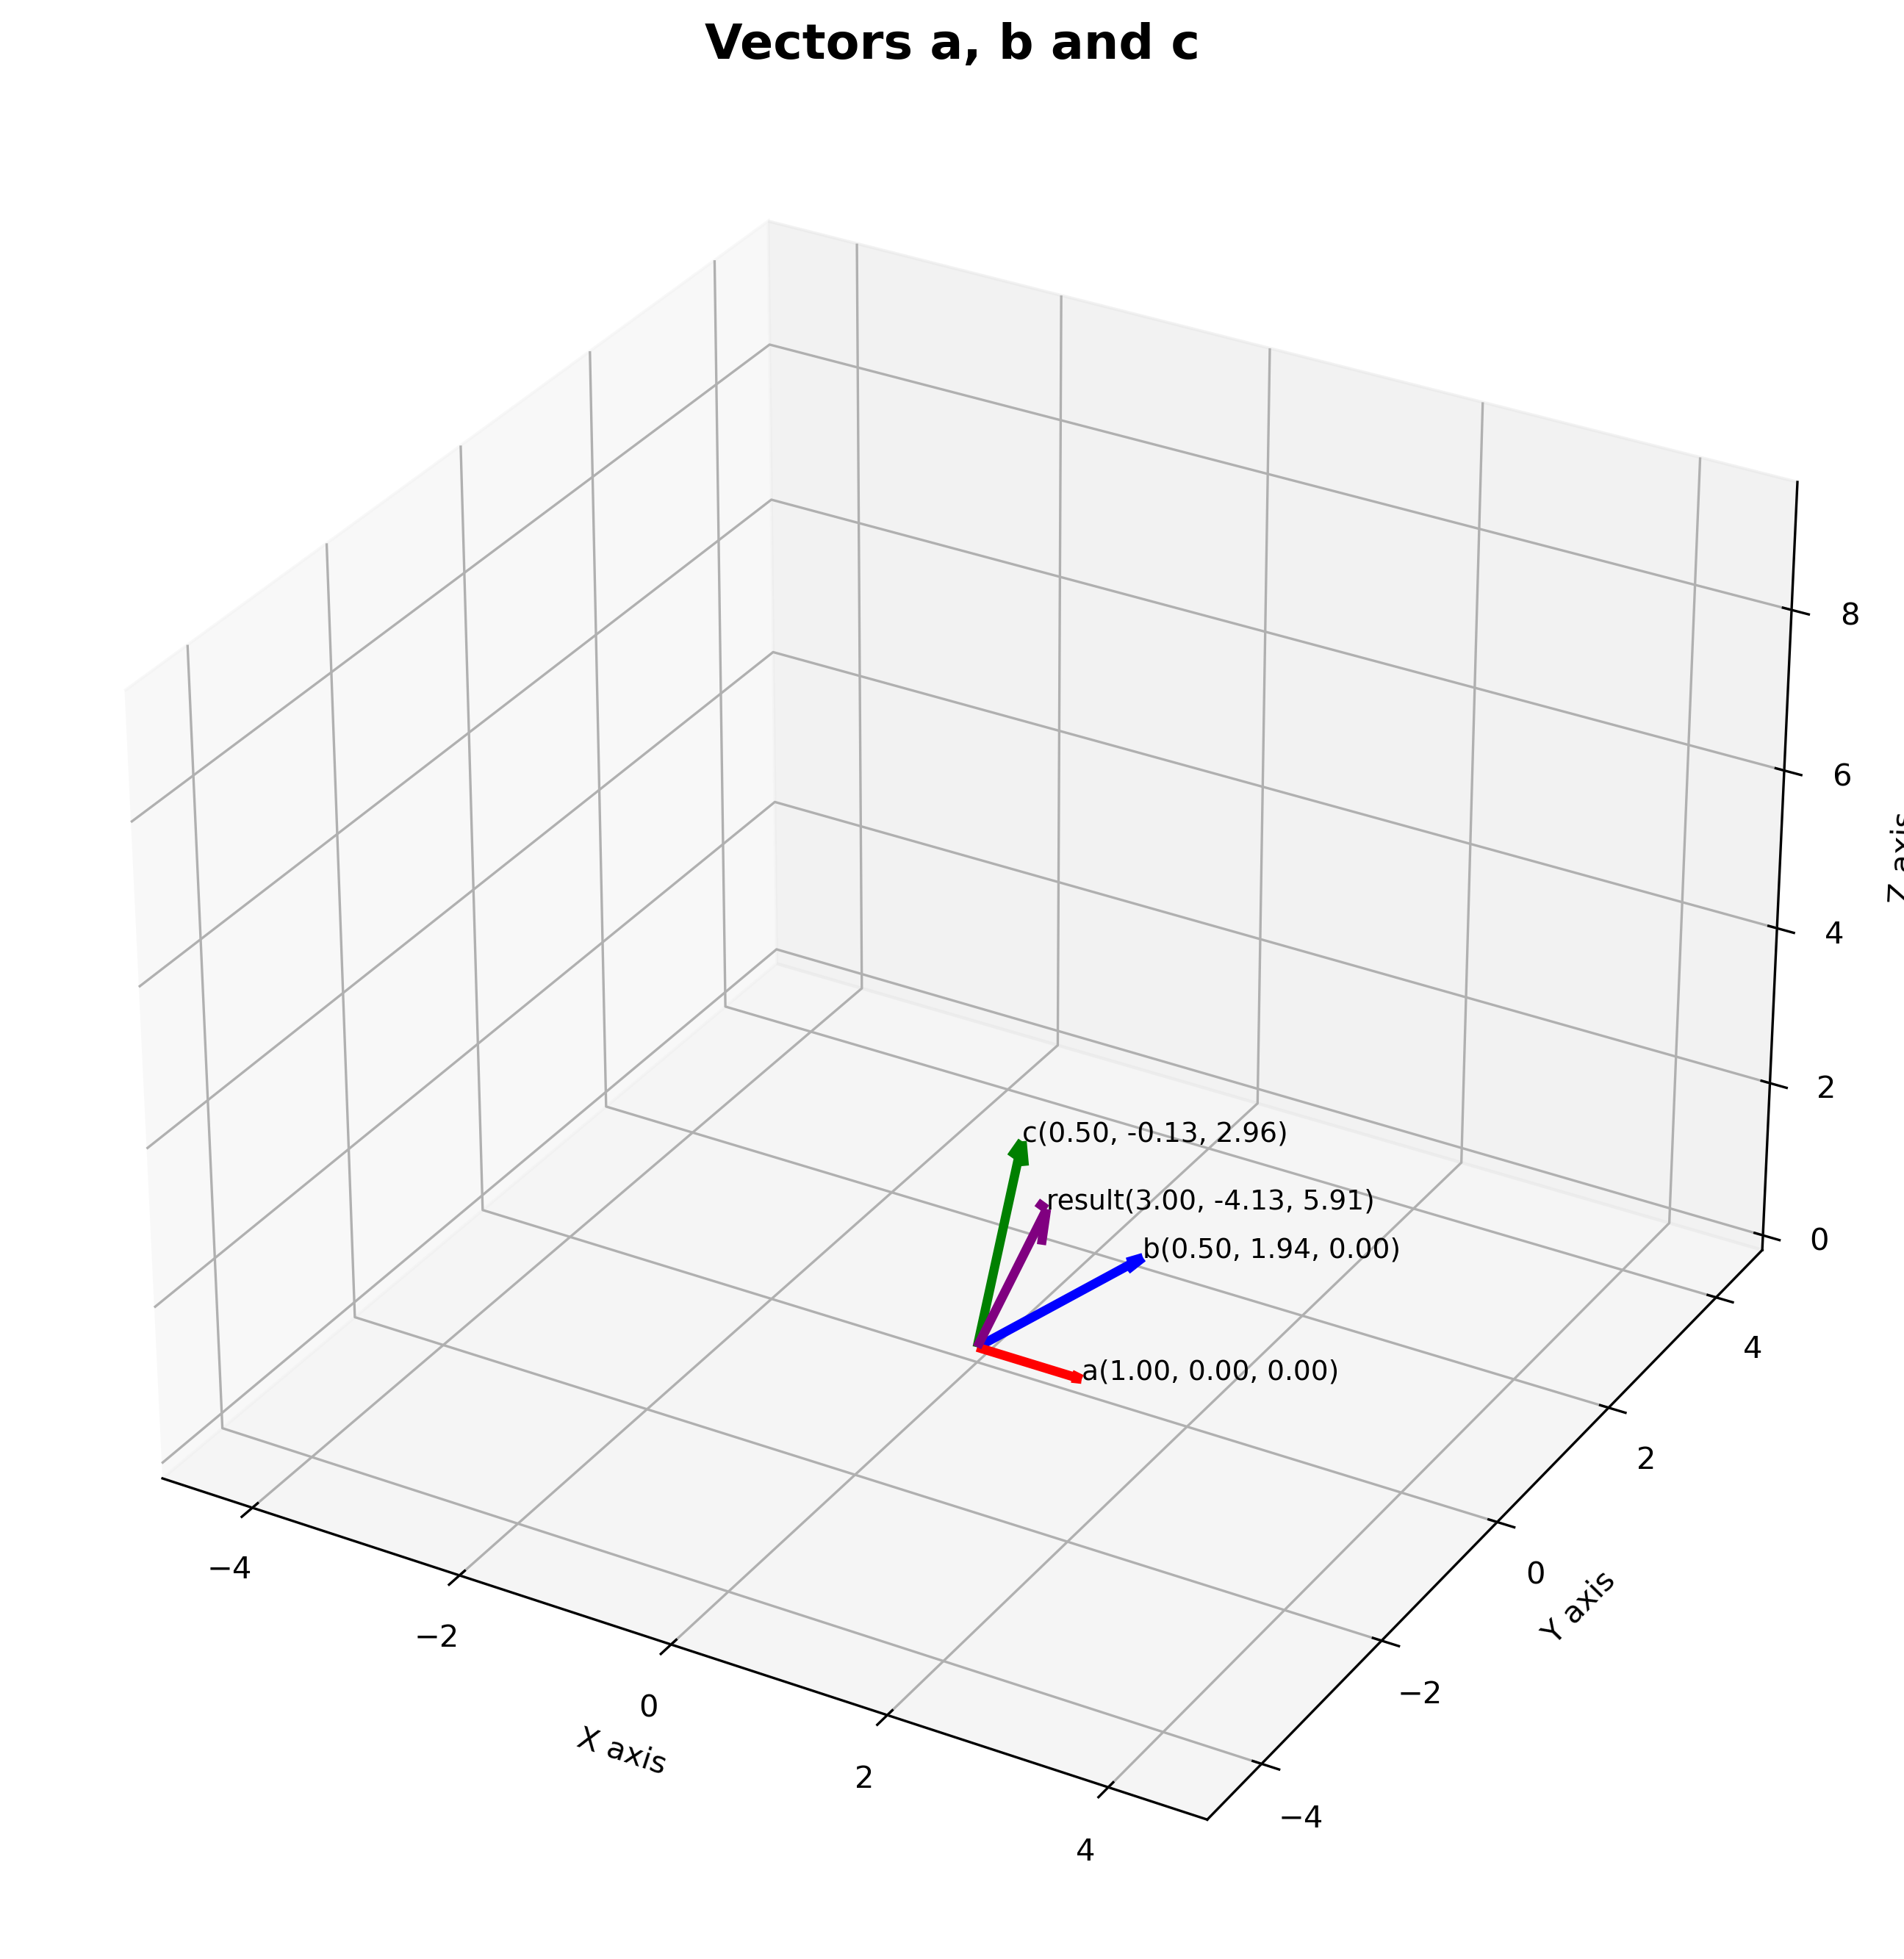
\includegraphics[width=\columnwidth, height=0.8\textheight, keepaspectratio]{figs/fig1.png}
    \label{fig:Beamer/figs/fig1.png}
\end{frame}


\end{document}